\documentclass[12pt,a4paper,oneside,english,brazilian,brazil]{abntex2}
% Para definir os idiomas e o tipo do documento.
\usepackage[T1]{fontenc}
% Para definir o tipo da fonte utilizada
\usepackage{arev}
% Para definir o tipo da fonte utilizada
\usepackage[utf8]{inputenc}
% Para exibir corretamente os caracteres especiais.
\usepackage{amsmath}
% Para a ferramenta matemática.
\usepackage{amssymb}
% Para símbolos Matemáticos.
\usepackage{amsfonts}
% Para fontes matemáticas.
\usepackage{mathtools}
% Para ferramentas matemáticas.
\usepackage{indentfirst}
% Para identação da primeira linha dos parágrafos.
    \setlength{\parindent}{1.25cm}
    % Para configurar (ABNT) identação de primeira linha.
    \setlength{\parskip}{0.2cm}
    % Para configurar (ABNT) distancia depois do parágrafo.
    \setlength{\headheight}{15pt}
    % Tamanho do cabeçalho do documento
\usepackage{graphicx}
% Para usar graficos.
    \graphicspath{imagens/}
    %Para definir uma pasta separada para imagens.
%\usepackage[round]{natbib}
% Para bibliografia.
%\usepackage[citestyle=authoryear,natbib=true,backend=bibtex]{biblatex}
% Para bibliografia.
\usepackage{hyphenat}
% Pacote para quebra de palavras e hifenação.
\usepackage{float}
% Para flutuar objetos na página.
\usepackage{scalefnt}
% Para modificar o tamanho das fontes.
\usepackage{booktabs}
% Para melhorar a qualidade de tabelas
\usepackage{longtable}
% Para tabelas de múltiplas páginas.
\usepackage{steinmetz}
% Para notação Steinmetz (\phase).
\usepackage{lscape} 
% Para formato de paisagem sem virar na visualização.
\usepackage{pdflscape} 
% Para formato de paisagem virando na visualização.
\usepackage{filecontents}
% Usa uma versão não integrada, permite a simulação de conteudo de outros arquivos diretamente deste.
\usepackage{pdfpages}
% Para inserir paginas de outros pdfs
\usepackage[alf,abnt-full-initials=no]{abntex2cite}
% Para usar o pacote de citações do abntex
\hypersetup{ % Para configurar os links
	colorlinks=true,	% Habilita a configuração de cor de links
	linkcolor=blue ,	% Cor do link
	citecolor=blue ,	% Cor da citação
	urlcolor=blue  }	% Cor da url

%---------------------------------------------
% Configurações globais 
%---------------------------------------------
\titulo{ Estudo de caso: \\Parsing sintático baseado em Autômatos Finitos Determinísticos }
\instituicao{Instituto Federal do Ceará}
\data{\today}
\local{Fortaleza}
\tipotrabalho{Trabalho}
\orientador{ Prof. Ernani Andrade Leite }
\coorientador{}
\autor{ DAVID PASSOS DE SOUSA \\ CARLOS DAVID LIRA \\FRANCISCO DAVI CAMILO RIBEIRO \\ EDBERTO LIMA DE ANDRADE \\ FILIPE RODRIGUES DE MENDONÇA }
\preambulo{Trabalho com o objetivo de obter menção na disciplina de Aspectos Teóricos para o curso de Engenharia de Computação do IFCE.}

% -------------------------------------------------
% Mantendo a bibliografia no mesmo arquivo
% -------------------------------------------------

\begin{filecontents}{bib.bib}

@book{  luger,
author = "George F. Luger",
title  = "Inteligência Artificial 6 Ed.",
subtitle = "",
volume = "",
year   = "2013",
month  = "",
note   = "",
publisher = "Pearson Education do Brasil",
address   = "São Paulo, SP"
}

@book{  trabaca,
author = "Gisele do Rocio Cordeiro, Nilcemara Leal Molina, Vanda Fatroti Dias",
title  = "Orientações e dicas práticas para trabalhos academicos",
subtitle = "",
volume = "",
year   = "2014",
month  = "",
note   = "",
publisher = "Editora Intersaberes",
address   = "Curitiba, PR"
}

@book{  model,
author = "Rodney Carlos Bassanezi",
title  = "modelagem matemática teoria e prática",
subtitle = "",
volume = "",
year   = "2015",
month  = "",
note   = "",
publisher = "Editora Contexto",
address   = "São Paulo, SP"
}

@book{  othero,
author = "Gabriel de Ávila Othero",
title  = "A GRAMÁTICA DA FRASE EM PORTUGUÊS",
subtitle = "ALGUMAS REFLEXÕES PARA A FORMALIZAÇÃO DA ESTRUTURA FRASAL EM PORTUGUÊS",
volume = "",
year   = "2009",
month  = "",
note   = "",
publisher = "EDIPUCRS",
address   = "Porto Alegre, RS"
}

@book{  othero2,
author = "Gabriel de Ávila Othero",
title  = "Teoria X-Barra",
subtitle = "Descrição do português e aplicação computacional",
volume = "",
year   = "2006",
month  = "",
note   = "",
publisher = "Editora Contexto",
address   = "São Paulo, SP"
}

@book{  esthum,
author = "Jack Levin, James Alan Fox",
title  = "Estatística para ciências humanas",
subtitle = "",
volume = "",
year   = "2004",
month  = "",
note   = "",
publisher = "PERSON Prentice Hall",
address   = "São Paulo, SP"
}

@book{  esteng,
author = "Ronald E Walpole, Raymond H. Myers, Sharon L. Myers, Keying Ye",
title  = "Probabilidade e Estatística",
subtitle = "para engenharias e ciências",
volume = "",
year   = "2008",
month  = "",
note   = "",
publisher = "PERSON Prentice Hall",
address   = "São Paulo, SP"
}

@book{  prolog,
author = "Eloi L. Favero",
title  = "Programação em Prolog",
subtitle = "uma abordagem prática",
volume = "",
year   = "2006",
month  = "",
note   = "",
publisher = "UFPA",
address   = "PA"
}

@book{  compiladores,
author = "Monica S. Lam, Ravi Sethi, Jeffrey D. Ullman",
title  = "Compiladores",
subtitle = "Princípios, técnicas e ferramentas",
volume = "",
year   = "2007",
month  = "",
note   = "",
publisher = "PERSON Prentice Hall",
address   = "São Paulo, SP"
}

@book{  matdiscreta1,
author = "Kenneth H. Rosen",
title  = "Matemática Discreta e suas Aplicações",
volume = "",
year   = "2009",
month  = "",
note   = "",
publisher = "AMGH Editora Ltda.",
address   = "São Paulo, SP"
}

@online{ 		  michaelis,
author			= "MICHAELIS",
title 			= "Dicionário de Português Online",
year			= "2015",
organization 	= "Editora Melhoramentos Ltda."
}

@online{ 		  wikibook,
author			= "WIKIPEDIA",
title 			= "Enciclopédia Online",
year			= "2016",
organization 	= "MUDAR ISSO AQUI DEPOIS"

}

@online{ 		  wiki:automatos,
author			= "WIKIPEDIA",
title 			= "Enciclopédia Online",
year			= "2016",
url             = "https://pt.wikipedia.org/wiki/Teoria_dos_au%C3%B4matos",
organization 	= "MUDAR ISSO AQUI DEPOIS"

}

@online{ 		  wiki:glc,
author			= "WIKIPEDIA",
title 			= "Enciclopédia Online",
year			= "2016",
url             = "https://pt.wikipedia.org/wiki/Gram%C3%A1tica_livre_de_contexto",
organization 	= "MUDAR ISSO AQUI DEPOIS"

}

@online{          sof:cfgVScsg,
author          = "Stackoverflow",
title           = "Context-free grammars versus context-sensitive grammars?",
year            = "2017",
url             = "https://stackoverflow.com/questions/8236422/context-free-grammars-versus-context-sensitive-grammars",
organization 	= "MUDAR ISSO AQUI DEPOIS"

}
\end{filecontents}

%-------------------------------------
% Capa personalizada
%-------------------------------------

\renewcommand{\imprimircapa}{%
	\begin{capa}%
	\center
	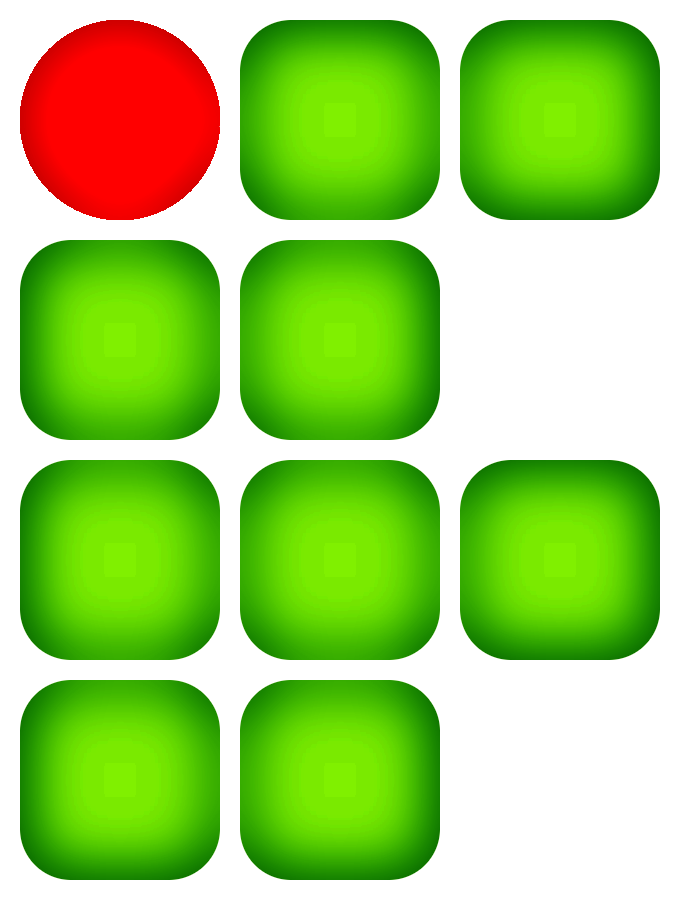
\includegraphics[scale=0.2]{Imagens/logo} \\
	\ABNTEXchapterfont\Large Instituto Federal do Ceará \\
	\vspace*{1cm}
	{\ABNTEXchapterfont\large\imprimirautor}
	\vfill
	\begin{center}
	\ABNTEXchapterfont\bfseries\LARGE\imprimirtitulo
	\end{center}
	\vfill
	\large\imprimirlocal \\
	\large\imprimirdata
	\vspace*{1cm}
	\end{capa}
}


%-------------------------------------
% Início do documento + Capa
%-------------------------------------
\begin{document}
\imprimircapa

%-------------------------------------
% Folha de rosto
%-------------------------------------
\imprimirfolhaderosto

%-------------------------------------
% Sumário
%-------------------------------------
\tableofcontents
\cleardoublepage % \clearpage ?

%-------------------------------------
% Resumo e Abstract
%-------------------------------------
%\begin{abstract}
%\par Este trabalho tem por finalidade apresentar a criação de um \textit{parser} sintático da gramática da língua portuguesa feito em java com foco na utilização de autômatos e aplicação em processamento de linguagem natural. \
%\textbf{Palavras-chave:} parser, java, autômatos, linguagem natural.
%\end{abstract}
%\pagebreak

% Abstract
%\selectlanguage{english}
%\begin{abstract}
%My abstract
%\end{abstract}
\selectlanguage{brazilian}
\pagebreak

%-------------------------------------
% Lista de figuras
%-------------------------------------
\pdfbookmark[0]{\listfigurename}{lof}
\listoffigures
\cleardoublepage

%-------------------------------------
% Lista de tabelas
%-------------------------------------
%\pdfbookmark[0]{\listtablename}{lot}
%\listoftables
%\cleardoublepage

%-------------------------------------
% Elementos textuais
%-------------------------------------
\textual

%-------------------------------------
% Capítulos e seções
%-------------------------------------
    
% Agradecimentos

% INTRODUÇÃO
\chapter{Introdução}

\par Este trabalho fala sobre uma biblioteca, escrita em java, que foi desenvolvida para analisar gramáticas regulares. Para tanto, levou-se em consideração os conhecimentos adquiridos das disciplinas Aspectos Teóricos, Inteligência Artificial  e no livro sobre Compiladores. Esta biblioteca serve como ponto de partida para outros trabalhos, como o de desenvolvimento de processadores de linguagem natural e compiladores. Os textos que descrevem como o trabalho foi realizado serão objetivos e enumerativos ao máximo, sem deixar de lado informações que sejam importantes para a reprodução deste, além disso, os exemplos serão extensivos e até prolixos, a finalidade é ter o maior numero de casos testados o possível, de tal forma que se possa comprovar a eficácia dos métodos utilizados. \

\par Assuntos relacionados ao trabalho ou à sua caracterização serão enumerados até que se convirja para o assunto principal. A ideia é convergir para se situar, de modo que cada passo seguido possa ser interpretado isoladamente e se necessário modificado para melhor entendimento, desempenho ou generalização do problema.\

\par Nos capítulos de 2 a 4 delimita-se o problema a ser tratado e suas aplicações, a solução proposta para sua resolução e os objetivos que norteiam o desenvolvimento do analisador sintático, além das dificuldades previstas pelas referências para o trabalho que se desenvolveu. \

\par Nos capítulos de 5 a 8 os assuntos que servem de embasamento para o entendimento do que se fez serão discutidos, as ferramentas utilizadas enumeradas, as soluções propostas e métodos utilizados descritas, o conjunto treinamento utilizado delimitado e, por fim, apresentam-se os resultados e conclusões obtidos ao longo do desenvolvimento. \

\pagebreak

\chapter{Problematização}


\par A necessidade de escrever um analisador (\textit{parser}) sintático surgiu juntamente com a vontade de se escrever um processador de linguagem natural (PLN). O analisador figura como um dos componentes mais importantes na construção de um PLN, pois ele é o elemento central que traduz a linguagem humana para uma interpretação computacional. O foco deste trabalho é, portanto, propor uma implementação do referido analisador.\

\par É desafiante desenvolver um analisador sintático para a língua portuguesa, pois os aspectos semânticos e exceções encontradas na língua acabam por tornar sua caracterização de difícil modelagem. Além disso, a língua portuguesa é extensa e o analisador precisa ser escrito de maneira a abarcar o maior número de casos o possível, caso contrário, não se poderia garantir a confiabilidade dos programas baseados na biblioteca proposta.\

\par A biblioteca desenvolvida propõe a implementação de uma gramática regular escrita sob os moldes da gramática normativa brasileira, proposta por Evanildo Bechara, apesar disto, ela não carrega consigo aspectos precisos a respeito da morfologia ou semântica, pois o objeto do trabalho ficaria demasiadamente extenso e o foco do desenvolvimento do analisador sintático seria perdido.\

\par Em razão  dos inúmeros problemas que existiram durante a fase de desenvolvimento do analisador, como sua caracterização extensa e por vezes ambígua, fez-se necessário utilizar alternativas para os códigos e regras gramaticais propostas, caso contrário não se teria um programa com solução precisa.\

\par Por fim, a solução para modelar um problema tradicionalmente da língua portuguesa em um ambiente puramente computacional consistiu na recorrência às técnicas de modelagem por autômatos, gramáticas regulares e expressões regulares, todos estes, presentes em alguma fase de desenvolvimento do código que aqui propomos, mas nem sempre tão fáceis de se perceber, mais difíceis ainda quando tiveram que ser abstraídos para integrar o código da linguagem de programação utilizada.\

\chapter{Objetivos}

\begin{itemize}
\item Criar o modelo diagramático do problema.
\item Criar o modelo diagramático do módulo (\textit{parser}).
\item Implementar o problema computacionalmente.
\item Melhorar a visualização do problema.
\item Justificar o uso da ferramenta computacional.
\item Justificar o uso dos aspectos teóricos para resolução do problema.
\end{itemize}

\chapter{Dificuldades e eventualidades}

Segundo o livro ``Inteligência Artificial'' \cite{luger} os seguintes problemas poderiam ocorrer durante a implementação do código do módulo.

\begin{itemize}
\item O problema das escolhas que levam à sentenças não interpretadas.
\item Dificuldade de controle da complexidade do problema.
\item Diferenças entre a implementação da \textbf{geração} \textit{versus}  \textbf{derivação}.
\end{itemize}

%\par Já segundo o livro ``Teoria X-Barra'' \cite{othero} poderiam ocorrer: \


%\par Segundo o livro ``Compiladores, Princípios, técnicas e ferramentas''.\cite{compiladores}. \



% CHAPTER
\chapter{Definições}

\section{A inteligência artificial}

\par Não há uma definição clara do que seja inteligência, portanto também não poderíamos definir o que é inteligência artificial de maneira precisa, contudo, numa tentativa de tornar claro o que se deseja com esse trabalho é preciso que se dê uma definição  formal para inteligência artificial que neste caso chamamos de ``parte da ciência que trata de sistemas inteligentes, capazes de se adaptar a novas situações, raciocinar, compreender relações entre fatos, descobrir significados e reconhecer a verdade.''. \cite{michaelis}. \

\par Desta ciência diversas áreas de estudo são concebidas e dentre elas se destaca o estudo sobre processadores de linguagem natural, objeto de estudo deste trabalho. \


\section{Processadores de Linguagem Natural (PLNs)}

Um do assuntos estudados pela Inteligência Artificial são os Processadores de linguagem natural. Estes não são um assunto novo, mas também não são um assunto de matéria já consolidada ou com pouco conteúdo. No livro ``Inteligência Artificial'' \cite{luger} podemos perceber que para se criar um processador de linguagem natural com capacidades para interagir com pessoas um série de assuntos merecem ser estudados, lá eles estão classificados por níveis de análise para linguagem natural:

\begin{itemize}
\item A prosódia.
\item A fonologia.
\item A morfologia.
\item \textbf{A sintaxe}.
\item A semântica.
\item A pragmática.
\item O conhecimento do mundo.
\end{itemize}

\par Embora hajam diversos assuntos pertinentes à inteligência artificial, neste trabalho, vamos nos ater apenas ao estudo e implementação do \textbf{analisador sintático} (\textit{parser} sintático), portanto, não se faz uma necessidade a definição de cada um dos níveis de análise dos PLNs, mas apenas este. \

\section{A sintaxe e o analisador sintático}



\begin{citacao}
``A Sintaxe estuda as regras para combinar palavras e sentenças válidas e o uso dessas regras para analisar e gerar sentenças. Esse é o componente de análise linguística que foi mais bem sucedida.''.\cite{luger}
\end{citacao}

\par A representação computacional da sintaxe se da por meio de gramáticas regulares, a sintaxe de que este trabalho se ocupa esta relacionada àquela que trata da organização dos \textbf{lexemas} na estrutura do que se chama de \textbf{período} (sentença), ou seja, embora objetivo principal deste trabalho seja ser fiel à gramática normativa e à analise sintática que esta faz, a construção de uma gramática operada por um autômato vai mais além, permitindo que também possa ser usada de modo genérico para outras aplicações computacionais. \

\begin{citacao}
``Regras de sintaxe são importantes não só em linguística, o estudo das linguagens naturais, mas também no estudo das linguagens de programação.'' \cite{matdiscreta1}.
\end{citacao}

\par Para tanto utilizou-se como base uma série de gramáticas e preceitos, de autores distintos, que integram a gramática proposta e implementada no módulo. Módulo este onde não delimita-se todos os casos linguísticos possíveis, pois o foco do trabalho seria perdido. \

\par Em seu livro de ``Inteligência Artificial'' \cite{luger}, o autor, explica: \


\begin{citacao}
``O primeiro estágio  é a análise (parsing), que analisa a estrutura sintática das sentenças. Ela verifica se as sentenças são sintaticamente bem formadas e determina, também, uma estrutura linguística. Identificando as principais relações linguísticas como sujeito-verbo, verbo-objeto, substantivo-modificador, o analisador fornece um arcabouço para a interpretação semântica, que normalmente é representado por uma árvore sintática. O analisador (parser) da linguagem emprega conhecimento sobre a sintaxe da linguagem, a morfologia e um pouco da semântica.''.\cite{luger}
\end{citacao}

\par Durante a fase de desenvolvimento do analisador também se faz necessário entender o papel das gramáticas regulares, mais especificamente das gramáticas dependentes (sensíveis) de contexto e de árvores de derivação, que constituem-se como ferramentas poderosas de modelagem de problemas envolvendo reconhecedores de linguagens. \

\section{Gramáticas Livres ou Sensíveis ao contexto}

Existem diversas classificações de gramáticas e para este trabalho só é importante saber que se utilizou uma gramática sensível ao contexto, contudo o conhecimento de algumas informações podem ser úteis. Considere as informações a seguir:

\begin{citacao}
``Toda gramática regular é livre de contexto, mas nem todas as gramaticas livres de contexto são regulares.''\cite{wiki:glc}.
\end{citacao}

\par Uma gramática é dita livre de contexto quando para cada estado S existe uma única regra de transição associada a partir de seu autômato correspondente e tal regra pode sempre ser utilizada. Já as gramáticas sensíveis ao contexto consideram a posição em que os elementos terminais ou não se enquadram na regra, veja um trecho encontrado em um fórum de grande credibilidade: \

\begin{citacao}
``A context-sensitive grammar (CSG) is a grammar where each production has the form wAx → wyx, where w and x are strings of terminals and nonterminals and y is also a string of terminals. In other words, the productions give rules saying "if you see A in a given context, you may replace A by the string y." It's an unfortunate that these grammars are called "context-sensitive grammars" because it means that "context-free" and "context-sensitive" are not opposites, and it means that there are certain classes of grammars that arguably take a lot of contextual information into account but aren't formally considered to be context-sensitive.''.\cite{sof:cfgVScsg}.
\end{citacao}

\par Entendido o que são gramáticas sensíveis ao contexto o resto do trabalho se torna de fácil compreensão e podemos continuar com a próxima ferramenta de modelagem importante, a árvore de derivação. \

\section{Árvore de derivação}

\par A árvore de derivação se constitui como uma árvore que representa as transições realizadas pelo analisador. Nela pode-se observar claramente as regras de derivação utilizadas, a raiz e os nós terminais para uma determinada análise.  \

\begin{citacao}
``Uma derivação na linguagem gerada por uma gramática livre de contexto pode ser representada graficamente usando uma árvore ordenada enraizada, chamada de árvore de derivação ou \textit{parse tree}.'' \cite{matdiscreta1}.
\end{citacao}


\par O interessante sobre essas árvores é que elas também podem ser modeladas por autômatos, de fato, o trabalho que se desenvolveu partiu de um autômato para se abstrair a busca em tal árvore. Essa abstração fica mais clara quando analisarmos o diagrama do autômato que foi desenvolvido nas páginas subsequentes. Por enquanto, é interesssante que se entenda também o que é o léxico. \

\section{O léxico}

\par O léxico que compõe este trabalho foi proposto inicialmente para o programa ``\textit{grammar play}'' \cite{othero2} e foi adaptado para seu uso pelo java, pouco tempo mais tarde, quando se viu que a abordagem feita por ele em \textit{prolog} seria melhor adaptada ao  autômato que se desenvolvia, então, o léxico foi alterado compondo não mais agora regras declarativas impostas pela linguagem de programação \textit{prolog}, mas uma implementação de um grafo escrito puramente em java.\

\par Alguns itens lexicais serão enumeradas abaixo a fim de que se possua um embasamento sobre o que foi feito, contudo, não podemos neste trabalho enumerar cada item gramatical, pois o léxico deste módulo é extremamente extenso. Veja: \

\setlength{\parindent}{0cm}
\hrulefill
\setlength{\parindent}{1.25cm}
\begin{verbatim}

 ama ,		  Verbo 
 amam ,		  Verbo 
 livros ,	  Substantivo 
 meninas ,	  Substantivo 
 amigo ,	  Substantivo 
 os ,		  Pronome 
 as ,		  Pronome 
 incrível ,	  Adjetivo 
 único ,	  Adjetivo 
 insubstituível , Adjetivo 
 má ,		  Adjetivo 
 da ,		  P 
 eu ,		  Pronome pessoal do caso reto 
 tu ,		  Pronome pessoal do caso reto 
 elas ,		  Pronome pessoal do caso reto 
 este ,		  Pronome demonstrativo 
 esta ,		  Pronome demonstrativo 
 algo ,		  Pronome indefinido 
 nada ,		  Pronome indefinido 
 como ,		  Adjunto 
 professor ,	  Substantivo 
 trabalho ,	  Verbo 
 estudo ,	  Verbo intransitivo 
 escreveu ,	  Verbo transitivo 
 é ,		  Verbo 
 português ,	  Substantivo 
 às ,		  Artigo 
 filho ,	  Substantivo 
 compreende ,	  Verbo 
 dos ,		  Pronome 
 pais ,		  Substantivo 
 esforço ,	  Substantivo 
 redação ,	  Substantivo 
 bela ,		  Adjetivo 
 esgotado ,	  Adjetivo 
 está ,		  Verbo de ligação 
 manhã ,	  Substantivo 
 prometia ,	  Verbo transitivo 
 chuva ,	  Substantivo 
 saíram ,	  Verbo 
 de ,		  Preposição 
 não ,		  Advérbio 
 foram ,	  Verbo 
 à ,		  Preposição 
 festa ,	  Substantivo 
\end{verbatim}
\setlength{\parindent}{0cm}
\hrulefill
\setlength{\parindent}{1.25cm}


\par Definido o léxico e a gramática tem-se quase tudo que é necessário para criar um analisador sintático, resta-se apenas então criar a lógica que opera os lexemas (palavras) a partir das regras gramaticais, e é aí que os autômatos finitos entram.

\section{Autômatos finitos (Máquinas de estados finitos)}

\par Um autômato é uma representação finita de uma linguagem formal que pode ser um conjunto infinito. Autômatos são frequentemente classificados pela classe das Gramaticas regulares (também conhecida como Tipo 3 da Hierarquia de Chomsky), é uma restrição sobre a forma das produções, pode-se criar uma nova classe de gramáticas de grande importância no estudo dos compiladores por possuírem propriedades adequadas para a obtenção de reconhecedores simples.\

\begin{figure}[H]
\centering
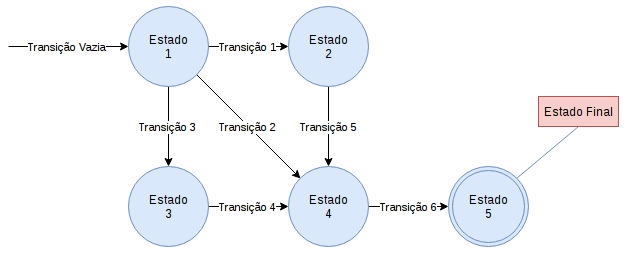
\includegraphics[scale=0.7]{Imagens/automatos.png}
\caption{Autômato Finito Definido}
\end{figure}

Ainda sobre autômatos, foi dito:

\begin{citacao} ``Na Ciência da computação teórica, teoria dos autômatos é o estudo dos objetos matemáticos chamados máquinas abstratas ou autômatos e os problemas computacionais que podem ser resolvidos usando esses objetos.'' \cite{wiki:automatos}. 
\end{citacao}

\par A justificativa para uso de autômatos se encontra no trecho a seguir:

\begin{citacao}
``(...) máquinas de estados finitos são a base para programas de verificação ortográfica, verificação gramatical, indexação ou busca em grandes textos, reconhecimento de fala, transformação de texto usando markup languages, como XML e HTML, e protocolos de redes que especificam como computadores se comunicam.'' \cite{matdiscreta1}
\end{citacao}

\par Diagramas de estados:

\begin{citacao}
``Outra maneira de mostrar as ações de uma máquina é usar um grafo com arestas rotuladas, em que cada estado é representado por um circulo, as arestas representam as transições e estão rotuladas com a entrada e a saída para aquela transição.'' \cite{matdiscreta1}
\end{citacao}

\section{Resumo definitivo}

A biblioteca criada neste trabalho utiliza-se de \textbf{regras de reescrita} para especificar uma \textbf{gramática sensível ao contexto} simbolizada por um conjunto de \textbf{cadeias não terminais}. Definimos também um \textbf{dicionário} formado por lexemas (nós terminais), para os quais assumimos que existirão \textbf{transições vazias} que formam a \textbf{raiz} da \textbf{árvore de derivação} em nosso \textbf{autômato finito definido}.

Este emaranhado de conceitos que inicialmente parece complicado, fica mais claro quando são mostrados por meio de \textbf{diagramas de autômatos} e por representações de \textbf{gramáticas}. Nestas representações também fica claro o uso de \textbf{regras de derivação} para uso no \textbf{analisador sintático}, bem como para conhecimento da utilização de um modelo \textbf{top-down} em detrimento do \textbf{botton-up} e vice-versa.

\par Definido tudo o que se precisava pode-se então ter a certeza de que a decisão de seguir uma gramática mais normativa e formal, como a proposta por Evanildo Bechara, é uma alternativa viável. Mostrar-se-á a seguir como se fez tal analisador.\

\chapter{Ambiente de desenvolvimento}

\par Mesmo simples, o projeto, foi desenvolvido ao longo de um tempo considerável e os softwares utilizados sofreram algumas modificações por seus fabricantes ao longo deste tempo, em sua versão mais atual o programa faz uso dos seguintes: \

\begin{enumerate}
	\item Netbeans IDE 8.2 (Livre)
	\item JDK 8u92 (Livre)
\end{enumerate}

\section{Configuração do ambiente de desenvolvimento}

\par Instalados todos os softwares acima listados é preciso configura-los. \

\subsection{JDK}

	\par O java development kit pode ser adicionado no caminho relativo a programas do windows ou linux (Path) em suas variáveis de ambiente, contudo esta opção é facultativa uma vez que a IDE pode ser configurada para reconhecer o caminho absoluto para suas bibliotecas. Lembre-se também de adicionar as bibliotecas de teste do jdk (Junit). \

\subsection{Netbeans}
	\par O netbeans foi escolhido por ser uma plataforma de desenvolvimento completa e bem recomendada pelos desenvolvedores da linguagem de programação java e depois de instalada basta que se configure-a para encontrar o JDK. Configuradas as bibliotecas faz-se necessário também que a biblioteca JUnit do java também se faça presente, este é um passo essencial e que costuma ser omitido, certificando-se que o JUnit foi configurado na IDE tudo ocorrerá bem.\
	
\subsection{O projeto em si}
	\par Na IDE em si basta que se crie um novo projeto e adicione os arquivos do projeto, desta forma, se o ambiente de testes do java estiver bem configurado o modulo será executado em modo de teste. \
	
\chapter{Implementação do Módulo}

\section{Lógica de funcionamento}

\par No núcleo do módulo implementou-se um método que é o código para um autômato, com sua legibilidade e interpretação tal qual deveria ser. Um conjunto de entrada que representa um estado e pode seguir por meio de regras de transição para novos estados e continuar esta busca até se atingir uma meta definida pela gramática. \

\vspace{1cm}
\begin{figure}[H]
\centering
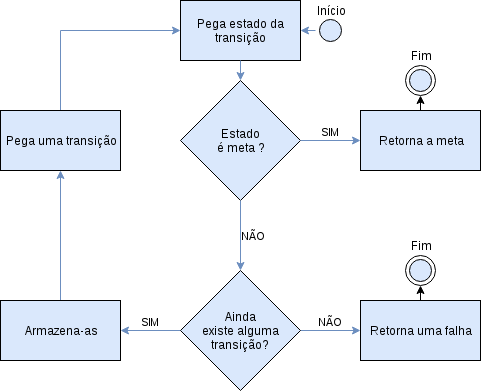
\includegraphics[scale=0.9]{Imagens/diagrama_analisador.png}
\caption{Modelo diagramático do analisador sintático.}
\end{figure}

\par Faz-se necessário tornar clara a ideia de que a gramática \textbf{não é o autômato em si}, o autômato não passa de uma abstração que faz o uso da gramática regular para consumir as entradas. \

\par O conjunto de entrada por sua vez é uma estrutura que relaciona um par de listas, do lado esquerdo o argumento de substituição e do lado direito a substituição em si. \

\section{Exemplo de uso}

\vspace{1cm}
\begin{figure}[H]
\centering
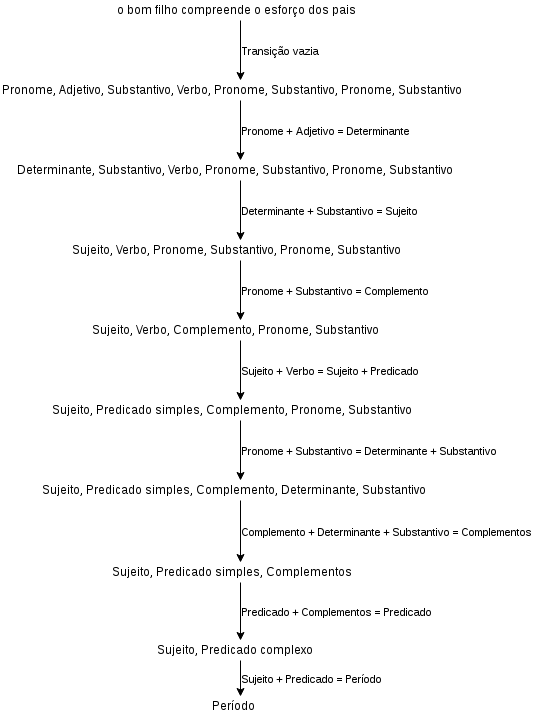
\includegraphics[scale=0.7]{Imagens/analise.png}
\caption{Modelo diagramático do caminho percorrido pelo analisador.}
\end{figure}

A imagem acima trata de como o programa analisa a estrutura sintática do período (sentença).

\section{``Conjunto treinamento''}

Utilizou-se para fins de experimentação da eficácia do módulo os seguintes conjuntos de entrada:

\setlength{\parindent}{0cm}
\hrulefill
\setlength{\parindent}{1.25cm}	
\begin{verbatim}
(CASO FAVORÁVEL) eu estudo português às segundas-feiras
(CASO FAVORÁVEL) eu estudo português
(CASO FAVORÁVEL) eu estudo
(CASO FAVORÁVEL) estudo
(CASO FAVORÁVEL) os homens desejam paz
(CASO FAVORÁVEL) eu trabalho como professor
(CASO FAVORÁVEL) muitas crianças viram os pássaros
(CASO FAVORÁVEL) o bom filho compreende o esforço dos pais
(CASO FAVORÁVEL) joão escreveu uma bela redação
(CASO FAVORÁVEL) o livro está esgotado
(CASO FAVORÁVEL) esta manhã prometia chuva
(CASO FAVORÁVEL) todos os alunos saíram
(CASO FAVORÁVEL) alguns de nós não foram à festa

(CASO DESFAVORÁVEL) casa a é bonita

\end{verbatim}

\setlength{\parindent}{0cm}
\hrulefill
\setlength{\parindent}{1.25cm}	

\section{Justificativa do uso de AFDs}
 
\par Inicialmente discutimos qual seria a melhor linguagem de programação para realizar a aplicação, de forma que fosse mais simples possível e que suas bibliotecas atendessem às necessidades de implementação da aplicação, inicialmente escolhemos o JAVA pois além da independência de plataforma possui extensa gama de bibliotecas que facilitam desenvolver este módulo.\

\par A partir da definição da linguagem utilizada, para o desenvolvimento da aplicação, precisamos avaliar uma expressão de entrada como gramatical ou não e isto foi feito utilizando-se conceitos de gramáticas regulares. Então dadas as facilidades inerentes à linguagem e a biblioteca ``regex'' já implementada por essa se justifica o uso de Java. \

\section{Problemas conhecidos}

\par Regras gramaticais mal formadas podem resultar em uma recursão infinita, o que faz com a máquina virtual java gere uma exceção de estouro de pilha (\textit{stackoverflow}). Para que isso não aconteça é necessário verificar se as regras de derivação geram estados convergentes e jamais cíclicos. \

\par Pode-se inserir também, inadvertidamente, outro problema à biblioteca, caso não se atente ao que esta sendo inserido às regras lexicais ou gramaticais. Sempre leve em consideração que a biblioteca é \textit{case sensitive}, isto é, diferencia minúsculas de maiúsculas, por isso, se o usuário não prestar atenção, o léxico ou a gramática podem acabar contendo regras não interpretáveis. Este erro é totalmente independente do programa e de difícil detecção.

\section{Resultados}


\par A implementação do módulo consistiu na criação de um método que se beneficiasse da ideia de consumo de estados de um autômato por meio de funções. \ 

\par O diagrama do autômato que serviu de embasamento para a criação do núcleo do programa já foi mostrado, em correspondência à ele o código implementado ficou da seguinte forma: \

\setlength{\parindent}{0cm}
\hrulefill
\setlength{\parindent}{1.25cm}
\begin{verbatim}
public Lista<String> busca( Lista<String> tokens )
    {
        if( tokens.equals( meta ) )return meta;
        for( Lista<String> transicao : transicoes( tokens ) )
            if( busca( transicao ).equals( meta ) )
                return meta;
        return new Lista<>( "Não é a meta" );
    }
\end{verbatim}
\setlength{\parindent}{0cm}
\hrulefill
\setlength{\parindent}{1.25cm}

\section{Gramática proposta}

Segue um exemplo de construção da gramática proposta

\setlength{\parindent}{0cm}
\hrulefill
\setlength{\parindent}{1.25cm}	
\begin{verbatim}
Sujeito, Predicado simples               
    -> Período
Verbo, Complemento                       
    -> Predicado simples
Predicado simples, Complemento           
    -> Predicado complexo
Verbo, Substantivo, Determinante         
    -> Verbo, Complemento
Verbo, Complemento, Complemento          
    -> Verbo, Complementos
Verbo, Complementos, Complemento         
    -> Verbo, Complementos
Verbo, Complemento, Complementos         
    -> Verbo, Complementos
Verbo, Adjunto, Substantivo              
    -> Verbo, Adjunto adnominal, Substantivo
Verbo, Adjunto adnominal, Substantivo    
    -> Verbo, Complemento
Verbo, Adjunto adverbial, Substantivo    
    -> Verbo, Complemento
Pronome, Substantivo, Verbo transitivo   
    -> Sujeito, Verbo transitivo
Pronome, Substantivo, Verbo intransitivo 
    -> Sujeito, Verbo intransitivo
Advérbio, Substantivo                    
    -> Determinante, Substantivo
Substantivo, Advérbio                    
    -> Substantivo, Determinante
Adjunto, Verbo                           
    -> Adjunto adverbial
Adjunto, Advérbio                        
    -> Adjunto adverbial
Adjunto, Adjetivo                        
    -> Adjunto adverbial
\end{verbatim}


\chapter{Limitações}

\par Entre algumas limitações que podemos citar estão:

\begin{itemize}
\item Não abarca todas as regras de sintaxe que poderiam ser escritas.
\item A gramática é dependente de contexto.
\item Não foram implementadas regras de concordância.
\item Não foram implementadas regras que tratem de pontuação.
\item Não foram implementadas regras que tratem de capitalização.
\end{itemize}

\par Em geral o programa está limitado aos verbetes que conhece, seu ``banco de dados''. O programa não é capaz aprender novos verbetes de uma forma "natural", pois este não se constituiu como foco de implementação, contudo o analisador que se descreveu pode ser atualizado, melhorado, embarcado, modificado para utilizações futuras. \

\chapter{Conclusão}

Percebe-se então que o algoritmo proposto segue os modelos já consagrados para a criação de analisadores sintáticos, o código ficou simples, robusto e escalável, uma vez que diversas novas regras poderão ser criadas para melhora-lo sem que se precise alterar diretamente a lógica das instruções propostas. Além disso, o código é portável e utiliza bem os recursos computacionais e da linguagem sob a qual foi escrita, fazendo com que possa ser utilizado na maioria das circunstâncias.



\chapter*{Apêndice A - Lista de sinônimos}
\addcontentsline{toc}{chapter}{Apêndice A - Lista de sinônimos}

\centering
\begin{tabular}{|l|l|l|l|}
\hline 
Léxico & Dicionário & & \\ 
\hline 
Analisador & \textit{Parser} & &\\ 
\hline 
Gramática & & &\\ 
\hline 
Item lexical & Palavra & \textit{Token} & Lexema\\ 
\hline 
Sentença & Período & &\\ 
\hline 
\end{tabular} 


% -------------------------------------------------
% Elementos pós-textuais
% -------------------------------------------------
\postextual

% -------------------------------------------------
% Bibliografia de fontes não citadas
% -------------------------------------------------

\nocite{trabaca}
%\nocite{luger}
%\nocite{trabaca}
%\nocite{model}
%\nocite{othero}
%\nocite{othero2}
%\nocite{esthum}
%\nocite{esteng}
%\nocite{prolog}
%\nocite{michaelis}
%\nocite{wikibook}

\bibliography{bib}

\end{document}